% --------------------------------------------------------------------------- %
%                       _           _
%   ___ ___  _ __   ___| |_   _  __| | ___
%  / __/ _ \| '_ \ / __| | | | |/ _` |/ _ \
% | (_| (_) | | | | (__| | |_| | (_| |  __/
%  \___\___/|_| |_|\___|_|\__,_|\__,_|\___|
% --------------------------------------------------------------------------- %
%*[ ]   fix chapter sub
\chapter{Conclusion}{}
\label{sec: conclusion}
\epigraph{\textit{`The image with which the artist works to realise his or her idea is no longer a phantom, it can be touched, navigated and negotiated with.'}}{\citep[p.5]{ryan1991}}

% \begin{figure}
%     \centering
%     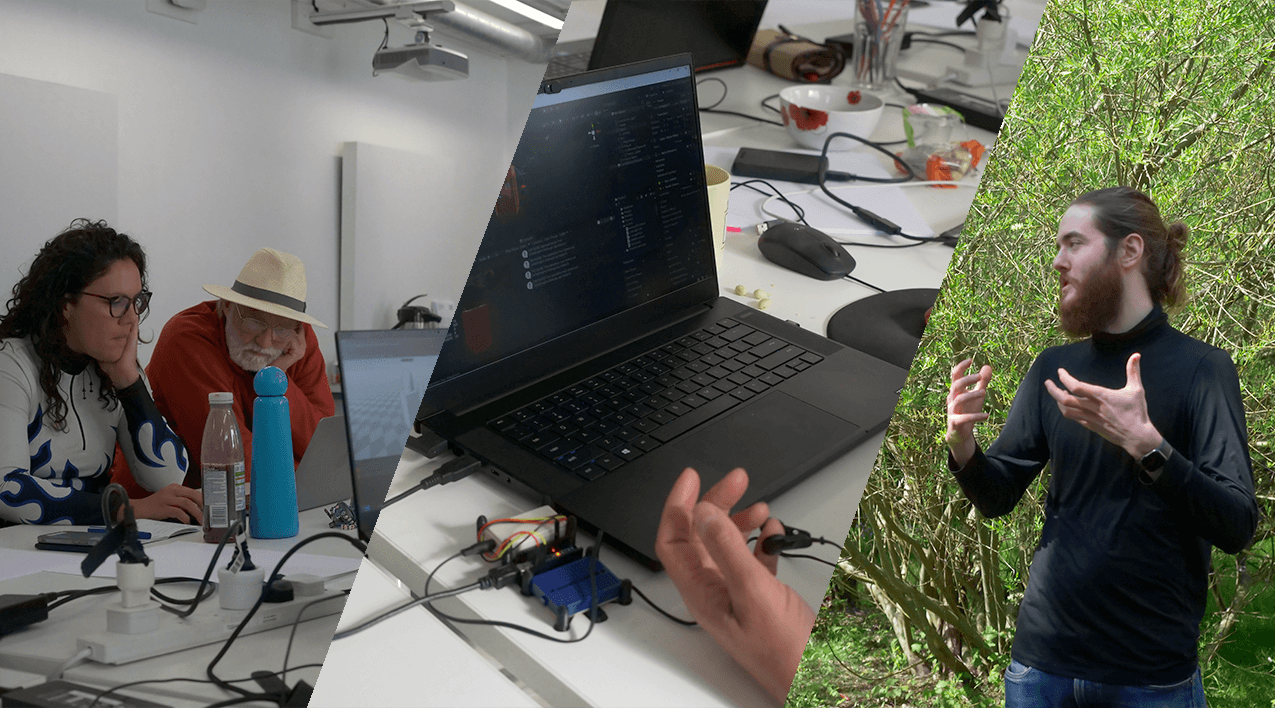
\includegraphics[width=1\linewidth]{0x-x/chapter-fig.png}
%     \captionsetup{labelformat=empty}
%     \caption[\autoref*{sec: x}'s page-figure: x, (from \citeauthor{x}, \citeyear{x})]{}
% \end{figure}

\clearpage
% --------------------------------------------------------------------------- %

\section{Summary}\label{sec: conclusion-summary}
There is no doubt, that \gls{ar} is one of the most exciting forms of technology on our horizon as artists and musicians. In this thesis, I hope I have portrayed this, with sufficient rationale, and explanation. However, there do exist significant problems; its origin in the U.S. \gls{mic}, as a tool for enabling neo-colonialism and the streamlining of workforces by increasing efficiency. Moreover, the threat of mega-corporations on our digital freedom, safety, and rights to privacy is beginning to surface in discussions regarding `the Metaverse' - the supposed site of \gls{xr} development. In stark contrast, federated and open communities like those that ActivityPub and Matrix provide, enable new and exciting ways to shift away from these platforms and the algorithmic harm they inflict. As such, \glshyperlink[open-source]{opensource} tools have provided much of the ability to carry out this research, and I would again like to thank those in the community that have helped: namely those involved in the \gls{pns}, LibPdIntegration teams.

The present thesis has presented three practical contributions to embodied musical knowledge and understanding in the form of \textit{\hyperref[sec: area]{area\textasciitilde{}}}, \textit{\hyperref[sec: polaris]{polaris\textasciitilde{}}}, and \textit{\hyperref[sec: polygons]{polygons\textasciitilde{}}}. In addition it has provided a set of three theoretical propositions, termed: augmented \hyperref[sec: discussion-medium-material]{materiality}, \hyperref[sec: discussion-medium-embodiment]{embodiment}, and \hyperref[sec: discussion-medium-space]{space} From this, design patterns for those in the field interested in reproducing or developing similar works, namely: \textit{\nameref{sec: discussion-patterns-experience}}, \textit{\nameref{sec: discussion-patterns-instrument}}, and \textit{\nameref{sec: discussion-patterns-environment}}, have been developed below.

% --------------------------------------------------------------------------- %
\section{Design Patterns for Sound ARt}\label{sec: discussion-patterns}
In \autoref{sec: method}, I outlined the primary vehicle through which to address the key topics and questions of the thesis: the creation and evaluation of sound \gls{art} experiences. These have, in their development and iteration, drawn on a proto-framework of implicit designerly tendencies and patterns that I have found effective - drawing from points of resistance (\autoref{sec: method-resistance}), and relevant perspectives from the field (\autoref{sec: theory}). In this section the aim is to outline these patterns in a way that may allow for the creation of similar works of \gls{art} in the future, by members of the experimental music, computational art, and digital humanities fields. The term design pattern here, is borrowed from the field of computer science, where it is taken to describe a set of `communicating objects and classes that are customized to solve a general design problem in a particular context' \citep{gamma1995}. A design pattern thus `names, abstracts, and identifies the key aspects of a common design structure that make it useful for creating a reusable object-oriented design'. So, while as a method it may not operate completely as it would in its native computer science, to address the outstanding aim of the thesis -- namely to contribute to the field of experimental music a guide to sound \gls{art} composition -- design patterns do serve to be less rigid than frameworks, more problem-focused than guidelines; whilst inheriting the meaningful organisational structure that comes with an object-oriented design approach. Design patterns are characterised by having four elements:
\begin{itemize}
    %*[ ]   first two look similar
    \item The \textbf{pattern name} describes the design problem at a higher level of abstraction
    \item The \textbf{problem} describes the specific situation in which you might apply the pattern
    \item The \textbf{solution} describes the relationships between elements of the pattern that aim to solve the problem
    \item The \textbf{consequences} are the results and trade-offs of applying the pattern
\end{itemize}

\begin{figure}
    \centering
    {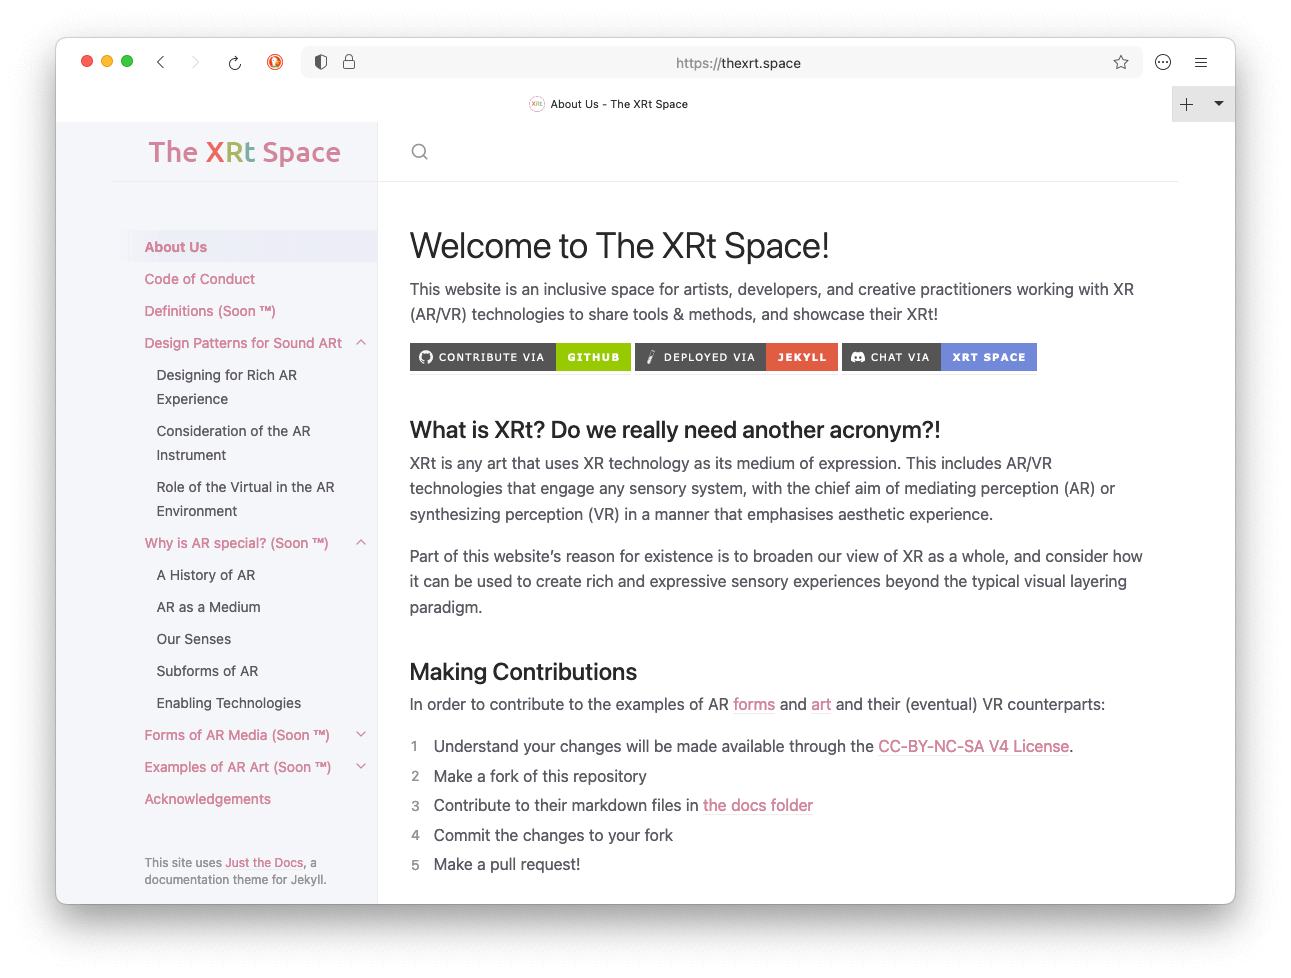
\includegraphics[width=.75\linewidth]{08-discussion/thexrtspace.png}}
    \caption[The XRt Space website]{The XRt Space website}
\end{figure}\label{fig: thexrtspace}

These design patterns are therefore subject to iteration, and the latest version can be found on \href{https://sambilbow.github.io/thexrtspace}{the XRt Space website}, a community-editable repository created to host and update them. The principles used to guide the patterns draw on the resistances outlined in \autoref{sec: method-resistance}, namely taking a \gls{diy} approach, decoupling from the ocularcentric and layering paradigms of typical \gls{ar} experience, and attempting to navigate an inherently consumerist space whilst trying not to contribute to exploitative systems of oppression that uphold it. They are also guided by the theoretical proposals of \autoref{sec: theory} and \autoref{sec: discussion-medium}: that participant's and performer's cognitive processes in the experience of \gls{ar} artworks are embodied, embedded, enacted, and extended, and have the potential to be modulated to extents that offer novel aesthetic experiences of augmented \hyperref[sec: discussion-medium-material]{materiality}, \hyperref[sec: discussion-medium-embodiment]{embodiment}, and \hyperref[sec: discussion-medium-space]{space}. The following sections outline three design patterns, \textit{\nameref*{sec: discussion-patterns-experience}}, \textit{\nameref*{sec: discussion-patterns-instrument}}, and \textit{\nameref*{sec: discussion-patterns-environment}}.

\subsection{Designing for Rich AR Experience}\label{sec: discussion-patterns-experience} 
\autoref{sec: theory} drew on a number of theoretical propositions, and put forward that \gls{ar} has the potential to scaffold new modes of performance and expression in the arts and music, furthermore, that from an enactivist approach experience, this would consist in radically modulating the material, embodied, and spatial experience of participants. This is the starting point for ideating and designing an artistic \gls{ar} experience in the present thesis. This pattern addresses the issue of the typicality of \gls{ar} experience being simple interactions with visual overlay devices. It approaches experience ideation from a holistic and multisensory, or `modalities-encompassing' \citep{schraffenberger2018} perspective. Furthermore, the \glshyperlink[`4Es' of an enactivist approach]{4ec} can be considered as conditions for what could be described as immersive and `rich experience' \citep{bilbow2021}. As highlighted in \autoref{sec: theory-materiality}, enactivist principles have been offered as guidelines for the creation of interactive systems in the past; Essl and O'Modhrain \citeyearpar{essl2006}, Armstrong \citeyearpar{armstrong2006}, and Hayes \citeyearpar{hayes2019} suggest this approach in the design of new musical instruments. 

The concept of rich experience also stands in stark contrast to the current direction of corporate \gls{xr} technologies, where it is being developed to \textbf{replace} in-person interactions e.g. by facilitating in-headset `work from home' \glspl{ve} such as Meta Horizons. It also stands in contrast with the marketed push towards \gls{ar} as a tool for driving commerce through targeted advertisements. How as artists and musicians can we avoid the corporate, commercial, ocularcentric, and overlay approach to \gls{ar}? How can we offset the dystopian hell-scape, painted by designer and film-maker Keiichi Matusda in various film shorts (see \autoref{fig: discussion-matsuda}).

\begin{figure}[hbt]
    \centering
    \captionsetup{justification=centering}
    \subcaptionbox{\textit{`The Pusher / The Entertainment'} \citep[from][]{matsuda2009}}[.45\linewidth]{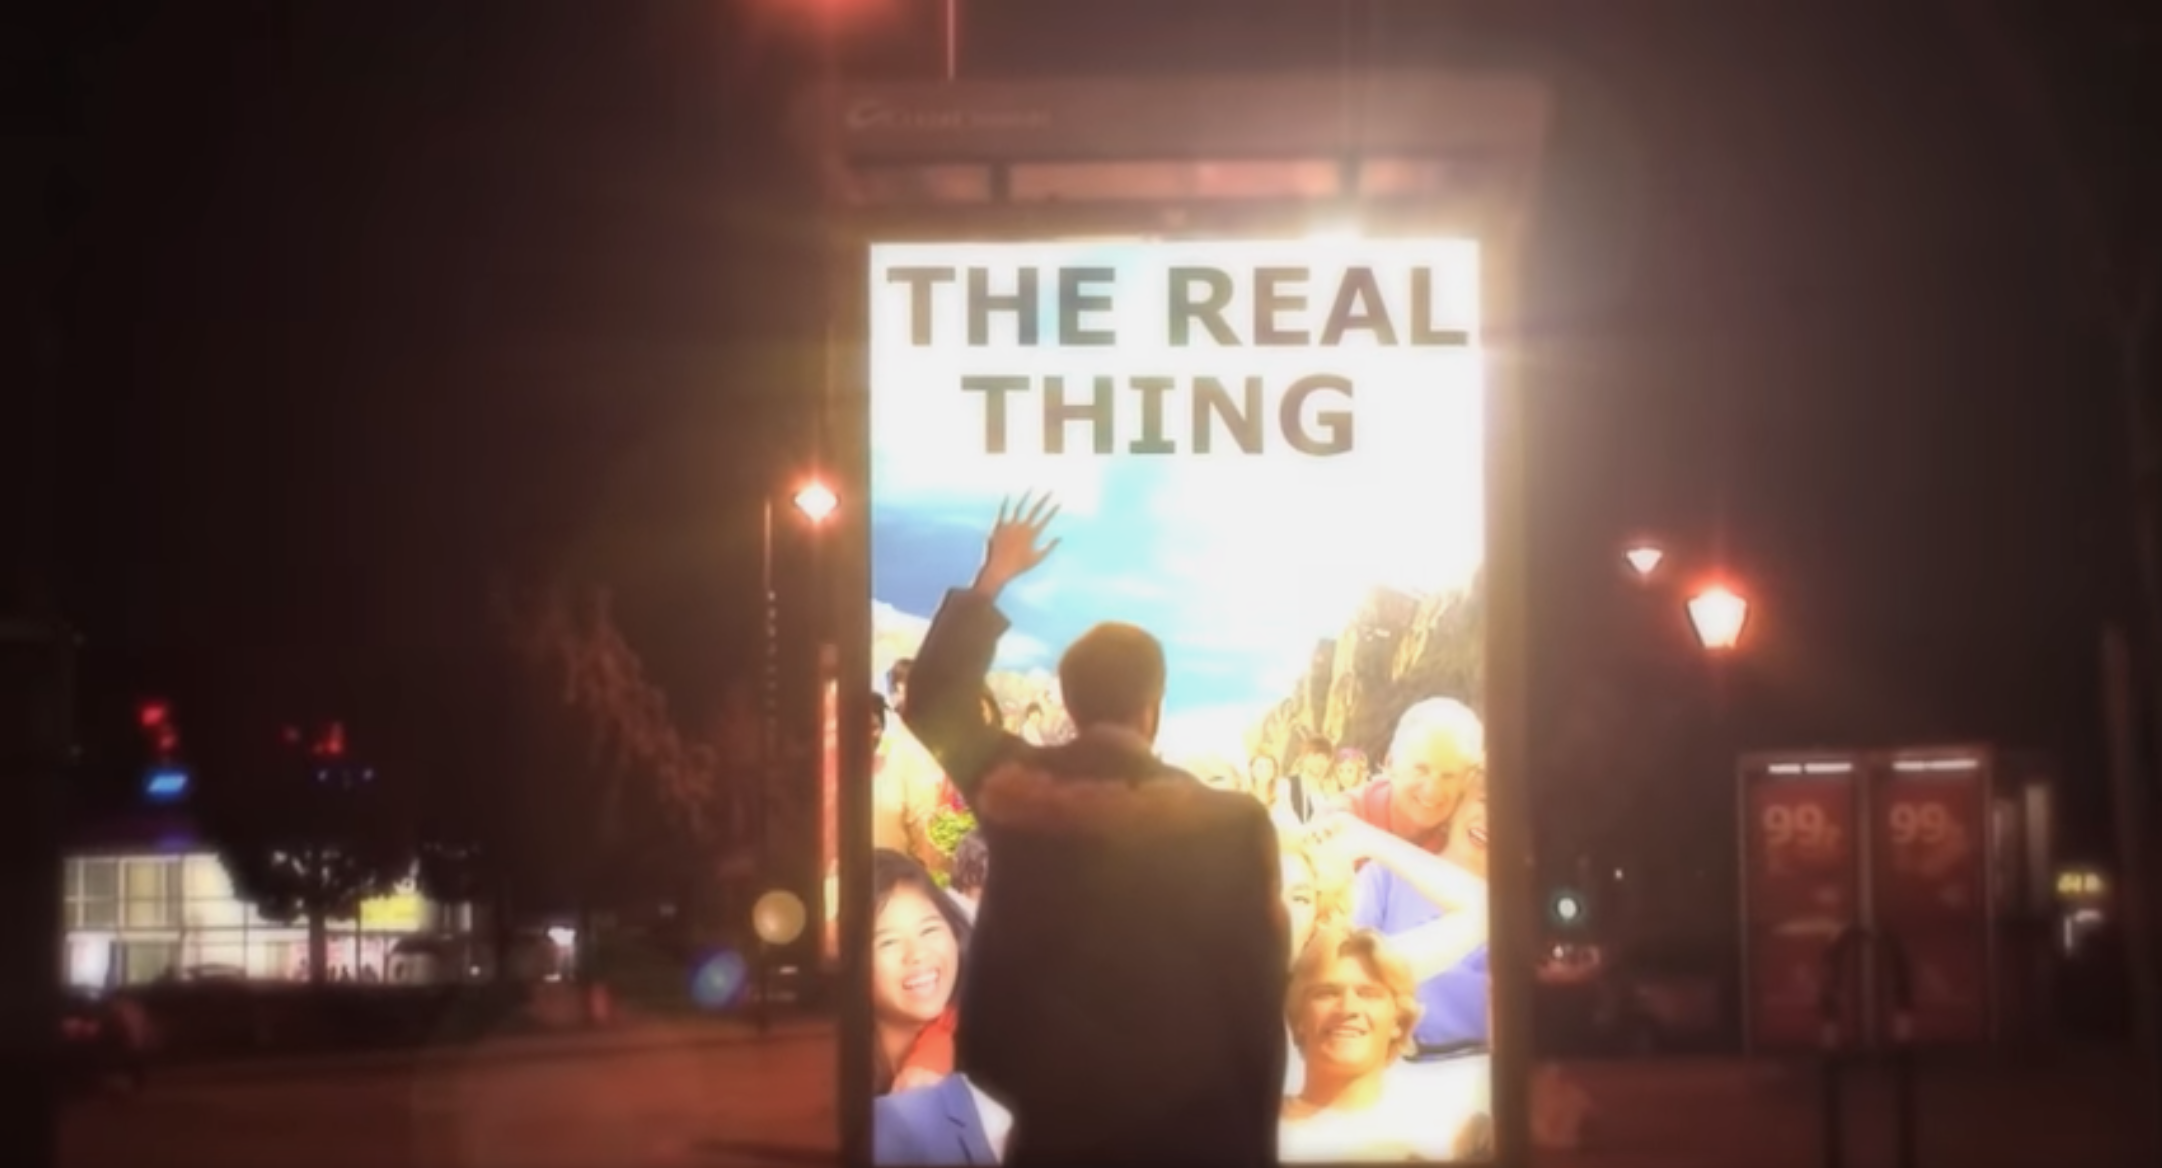
\includegraphics[height=3.8cm]{08-discussion/matsuda2009.png}}
    \hfill
    \subcaptionbox{\textit{`Augmented (hyper)Reality: Domestic Robocop'} \citep[from][]{matsuda2010}}[.45\linewidth]{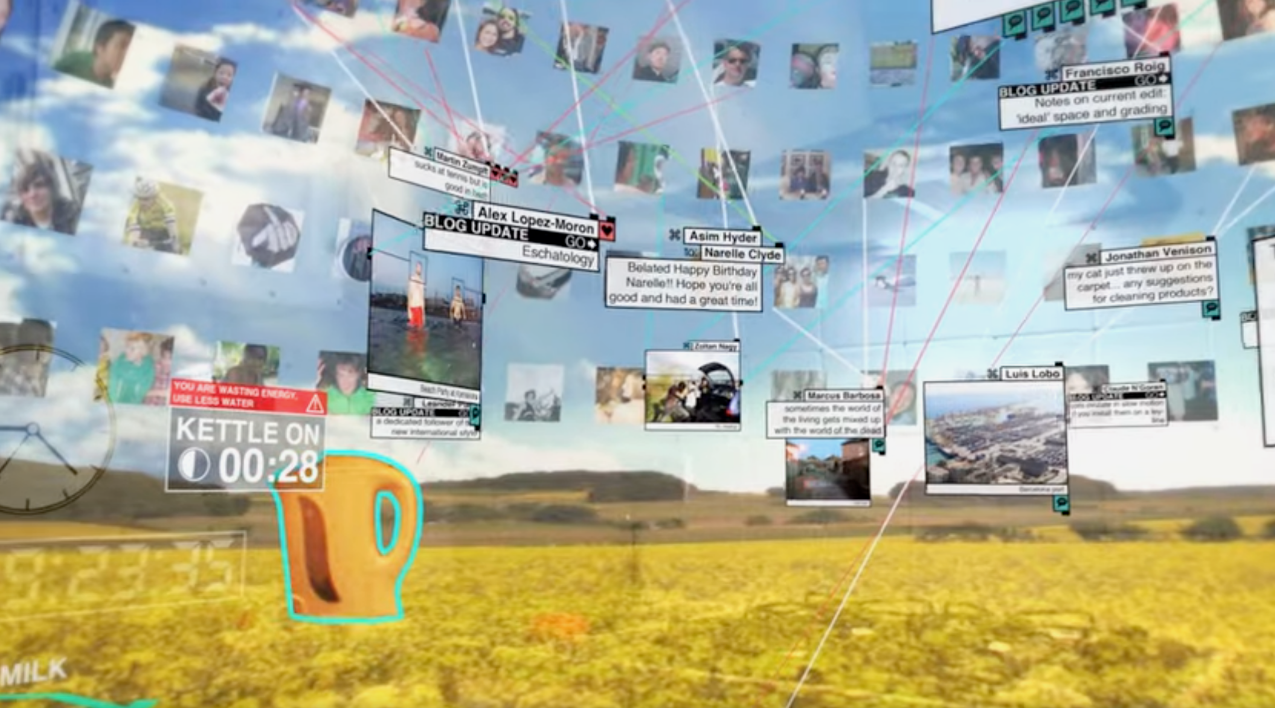
\includegraphics[height=3.8cm]{08-discussion/matsuda2010.png}} \\
    \vspace{0.5cm}
    \subcaptionbox{\textit{`HYPER-REALITY'} \citep[from][]{matsuda2016}}[.45\linewidth]{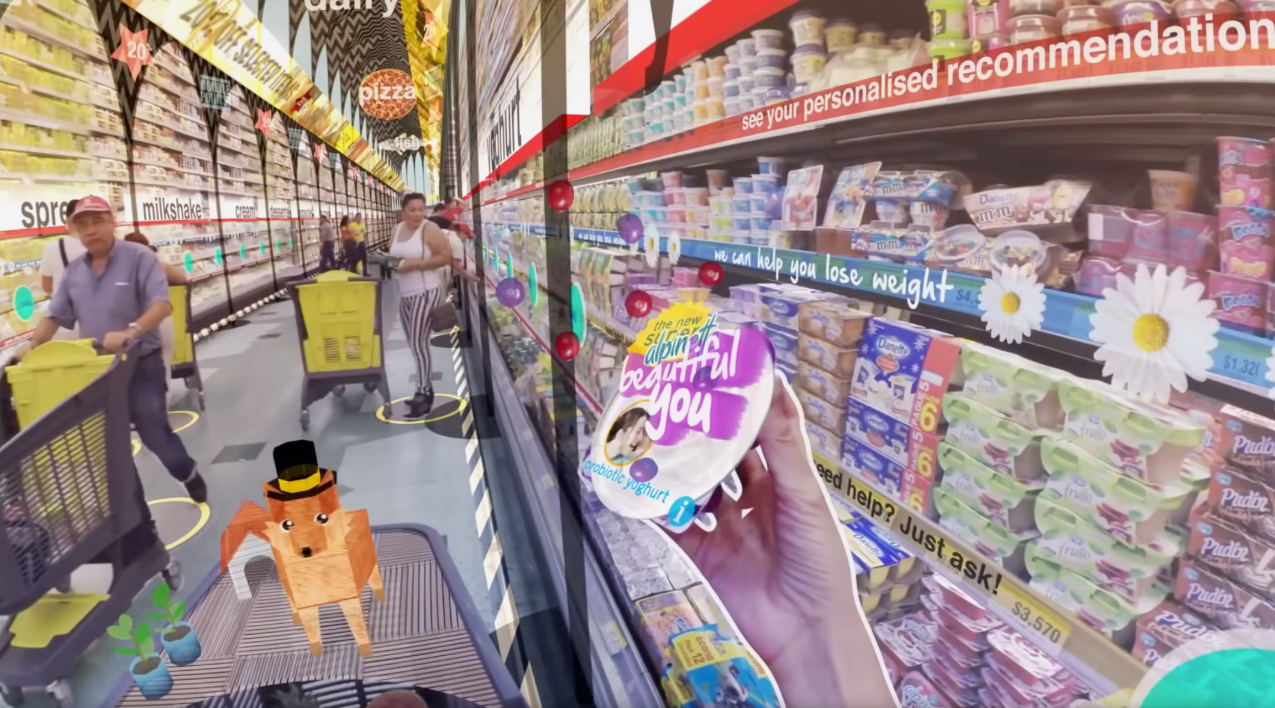
\includegraphics[height=3.8cm]{08-discussion/matsuda2016.png}}
    \hfill
    \subcaptionbox{\textit{`Merger'} \citep[from][]{matsuda2019}}[.45\linewidth]{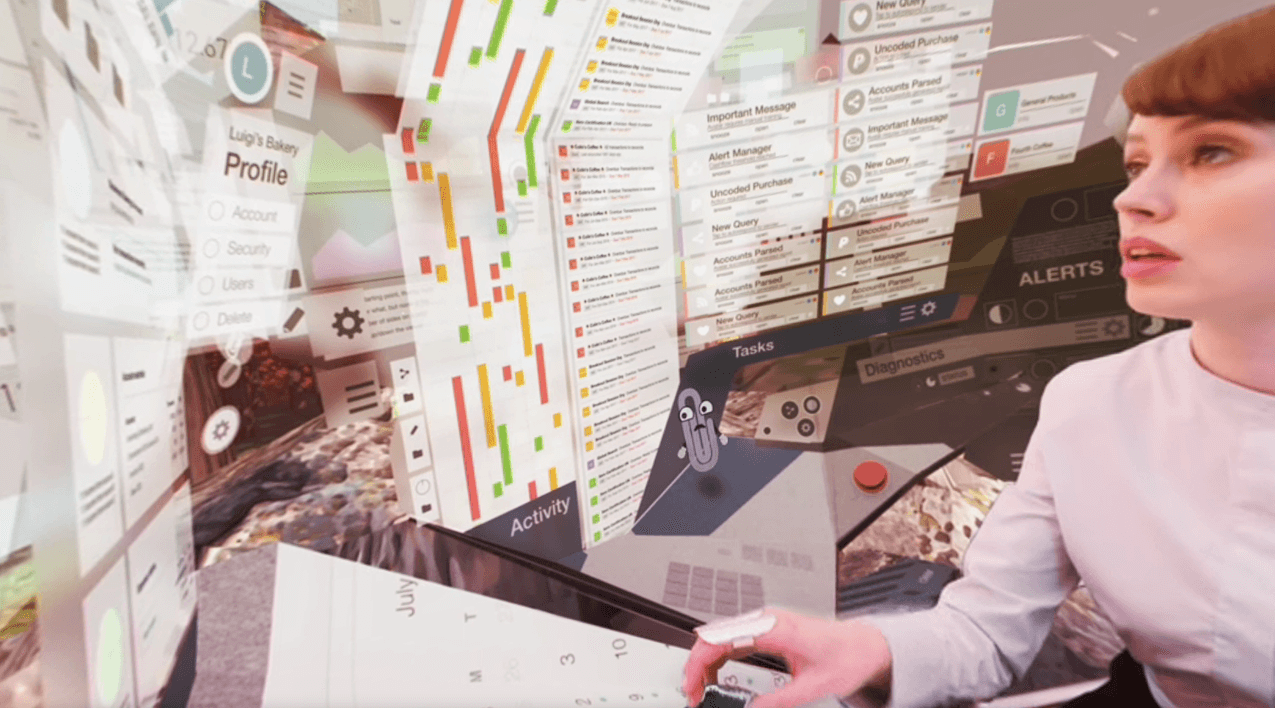
\includegraphics[height=3.8cm]{08-discussion/matsuda2019.png}}
    \caption{Keiichi Matusda's short films on dystopian AR futures}
    \label{fig: discussion-matsuda}
\end{figure}

\subsubsection{Centre the experience on two or more sensory interactions}
Whether it is Dewey's concept of the `live creature', or the contemporary enactivist's framing of the importance of embodiment, the \gls{ar} experience ought to be \textit{centred on two or more sensory interactions}. It may include any combination of sensory interaction (display or sensing) types, e.g. visual (vision), auditory (hearing), vestibular (movement and balance), olfactory (smell), gustatory (taste), and somatosensory (touch). This ensures grounding in the importance of the participants agency and sensorimotor structure. Here, the importance of considering the \gls{ar} experience as an enaction, rather than an abstract internal representation that they are thinking and then acting upon is the important.

\subsubsection{Invoke a meaningful relationship between the real and virtual}
\gls{ar}'s medium specificity, discussed in \autoref{sec: discussion-medium-material}, should be at the forefront of intentional design choices. If \gls{ar} is unique because of its `invocation of relationships between real and virtual processes in the axes of spatial, thematic, material and ecological distance', these relationships become a key handle by which artists and musicians can \textit{meaningfully steer experience to achieve aesthetic experiences}. Consider the following:
\begin{itemize}
    \item Spatial: to what extent should the virtual and real be spatially aligned or even spatially related?
    \item Thematic: to what extent should the virtual and real be thematically similar, what effect might this have on participants' sense of sensory congruency if distant instead?
    \item Material: to what extent should the virtual be materially similar to the real environment in which \gls{ar} brings it into conversation with? 
    \item Ecological: to what extent should the virtual act as part of the real environment, how does this suit the overall narrative intention of the piece?
\end{itemize}
For the artist or musician, the interest and specificity of \gls{ar} might lend itself to tending towards the revealing the differences rather than the similarities between the virtual and the real!

\subsubsection{Implement an AR subform}
In considering the embodied experience of participants, employ Schraffenberger's taxonomy of \gls{ar} subforms. As discussed in \autoref{sec: discussion-medium-embodiment}, augmented embodiment is achieved through the fact that \gls{ar} has the potential to radically modulate a participants sense of self, other, and environment. The present thesis has made a clear standpoint on the role of the \gls{mic} in biasing the development and conceptualisation of \gls{ar} towards that of an overlay device or heads-up display. Artists and musicians engaging in \gls{ar} will already be tending towards the altered and hybridised subforms of \gls{ar} rather than the purely augmenting; but it is worth mentioning here that significant improvements in the effectiveness of \gls{ar} in delivering aesthetic experience lies in considering the \textit{process} (see subform) by which perception is mediated by \gls{ar}.

\subsection{Consideration of the AR Instrument}\label{sec: discussion-patterns-instrument}
When describing the means through which a participant or performer meaningfully interacts or engages in any kind of information transfer in the \gls{ar} system, it is through what could be termed the \gls{ar} Instrument. The following categorisation (see \autoref{table: ar-instrument}) may be helpful in considering the plethora of different options available for artists and musicians.
%*[ ]   Replace with LaTeX table
\begin{table}
    \centering
    {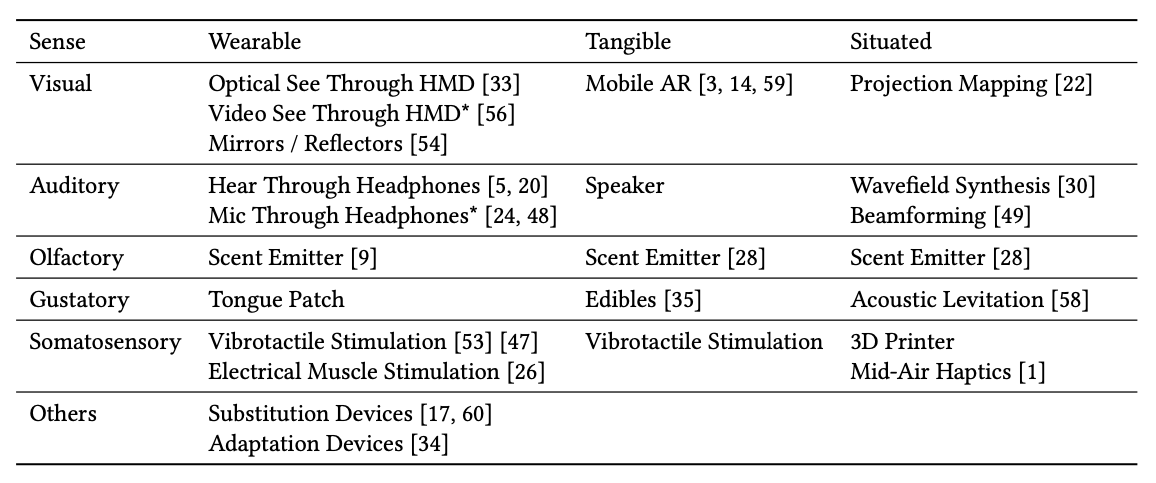
\includegraphics[width=1\linewidth]{04-method/sensorydisplays.png}}
    \caption[Potential AR Instruments]{Potential AR Instruments}
\end{table}\label{table: ar-instrument}

\subsubsection{Wearable}
Wearable \gls{ar} Instruments include forms that are worn on the body, including output via head-mounted visual, audio, olfactory and gustatory feedback devices or `displays', and body-mounted proprioceptive feedback devices

\subsubsection{Tangible}
Tangible \gls{ar} Instruments include forms that can explored by holding or touching, such as devices that use conductive fabrics and textiles to track input, and then providing sensory feedback, e.g. vibrotactile stimulation (somatosensory). They can also be any object that can be granted instrumentality by a device that can track it and provide contextually aware, i.e. corresponding, sensory feedback via another device. For example, a wooden cube could be transformed into a Tangible Instrument through real-time image recognition, and specific interactions with it could provide auditory feedback. In this example, the auditory feedback would likely be delivered via a Wearable Instrument that was also processing the real-time image recognition such as an \gls{hmd} with bone-conduction headphones.

\subsubsection{Situated}
Situated \gls{ar} Instruments include forms that are anchored in a real world environment and therefore provide location-specific experiences. Activation is gauged by user enaction, or user presence via infrared camera tracking or proximity of a worn device. Examples of Situated \gls{ar} Instruments could include an interactive projection mapping with wavefield synthesis providing auditory feedback, and anchored scent emitters providing olfactory feedback

\subsection{Role of the Virtual in the AR Environment}\label{sec: discussion-patterns-environment}
\subsubsection{Allowance for the Real}
The use of the game engine Unity, and visual programming languages like \gls{pd} / Max MSP have been invaluable in the development of the three outlined sound \gls{art} experiences. Thinking about how they integrate with the real environment of your participant is how \gls{ar} stays distinct from \gls{vr} on an interaction level - after all, there must be some reason why as an artist or musician, we decide to work in tandem with, rather than shut off, the real world from our participants! Consider the following:
\begin{itemize}
    \item What are the sensory boundaries implicit in both the real and virtual space I'm using? 
    \item What different sensory affordances are provided by both the real and virtual environments? 
    \item How might the development of augmented material be influenced by the above factors?
    \item What real objects are present in the space, is this intentional?
\end{itemize}

\subsubsection{Choosing Experience Size and Complexity}
It may be helpful to distinguish between different types of \gls{ar} `experience sizes' when first starting out developing sound \gls{art}. For doing this, I developed the following three categorisations. Implying or explicitly stating these boundaries (if it is a public installation) is necessary for building trust and ensuring safety. Intentionally setting boundaries may help in the creative process too.

Snippets describe a small-scale clip-like \footnote{Similar in scale to the video-clip, sound-clip, clipart, and now app-clip, however conceptually different in that Snippets are not a miniaturised `extracts' or `segments' of a larger experience} \gls{ar} Experiences that occur in the approximate interaction space of 30cm3, e.g. between a users hands. The Snippet itself does not supply a full sensorial experience, instead providing two human-to-sense interactions through its \gls{ar} subforms.

Scenes describe medium-scale \gls{ar} Experiences that occur on and around the body, an approximate interaction space of 200cm3. They can be formed from existing Snippets, or created from scratch. They ideally feature more (and higher complexity) human-to-sense interactions, and therefore potentially more interactive relationships between real and virtual elements will be formed.

Spaces describe large-scale \gls{ar} Experiences, involving multiple participants in a variety of differently sized interaction spaces in a room. For example, augmented hand / body interaction with the environment and other users, and multiple of zones of interaction in different sections of the space. Spaces provide fully multisensory immersive experiences, by making use of a combination of different sensory modalities and \gls{ar} subforms.



\section{Future Work}\label{sec: conclusion-futurework}
It is my hope to carry on developing expressive tools for musical creativity long into the future, and these will be located on \href{https://sambilbow.com}{on my website}. In \textit{\nameref{sec: polygons}}, I remarked on the work that was outstanding in developing a sound \gls{art} performance practice. It is my hope in the near future, to develop a set of tools for artists and musicians interested in collective forms of \gls{ar} headset expression, with a project entitled CoMuSe: Collective Musical Sensehacking. This will explore `multiplayer' or ensemble sound \gls{art} performances.
